\subsection{Grundkonzept des Benutzeroberflächen-Design}
\label{subsec:grundkonzept-des-benutzeroberflachen-design}

In diesem Abschnitt soll das Grundkonzept der Benutzeroberfläche beschrieben und dargestellt werden.

Die Benutzeroberfläche wird in drei Seiten aufgeteilt, welche sich mit dem Einlesen der Daten, dem
darstellen und auswählen zu visualisierenden Daten und dem Ausgeben das Ergebnis befasst.
Für das Navigieren zwischen den Seiten soll sich auf jeder Seite eine Navigation-Menü im oberen Bereich
der Seite befinden. Zudem sollen alle Seiten einen Bereich für Systemnachrichten wie Bestätigung oder

Fehlermeldungen und ein Label für die Seitenüberschrift besitzen. Diese soll direkt unter den Navigation-
Menü angesiedelt werden, um die Grundstruktur identisch aufzubauen. In den nachfolgenden Text werden
die Konzepte der Benutzeroberflächen und ein grundlegendes Benutzungskonzept der einzelnen Seiten
anhand der Abbildungen \ref{fig: Benutzeroberflächenentwurf der Seite zum Einlesen der XML-Struktur},
\ref{fig: Benutzeroberflächenentwurf der Seite zum Ausgeben der Berichtstabelle} und \ref{fig: Benutzeroberflächenentwurf der Seite zum Ausgeben der Graphen} beschrieben.

Für das Einlesen der XML-Daten soll ein Eingabebox genutzt werden, in die die XML-Struktur kopiert wird.
Die Eingaben soll über einen Button unter der Eingabebox bestätigt werden. Bei einem erfolgreichen
Einlesen und einfügen in die Datenbank soll eine Bestätigungsnachricht im Bereich für
Systemnachrichten erscheinen. Bei einem Fehler soll in diesem Bereich eine Fehlermeldung mit
möglicher Lösung erscheinen. Der Aufbau dieser Seite ist in der Abbildung \ref{fig: Benutzeroberflächenentwurf der Seite zum Einlesen der XML-Struktur} dargestellt.

\begin{figure}[H]
    \centering
    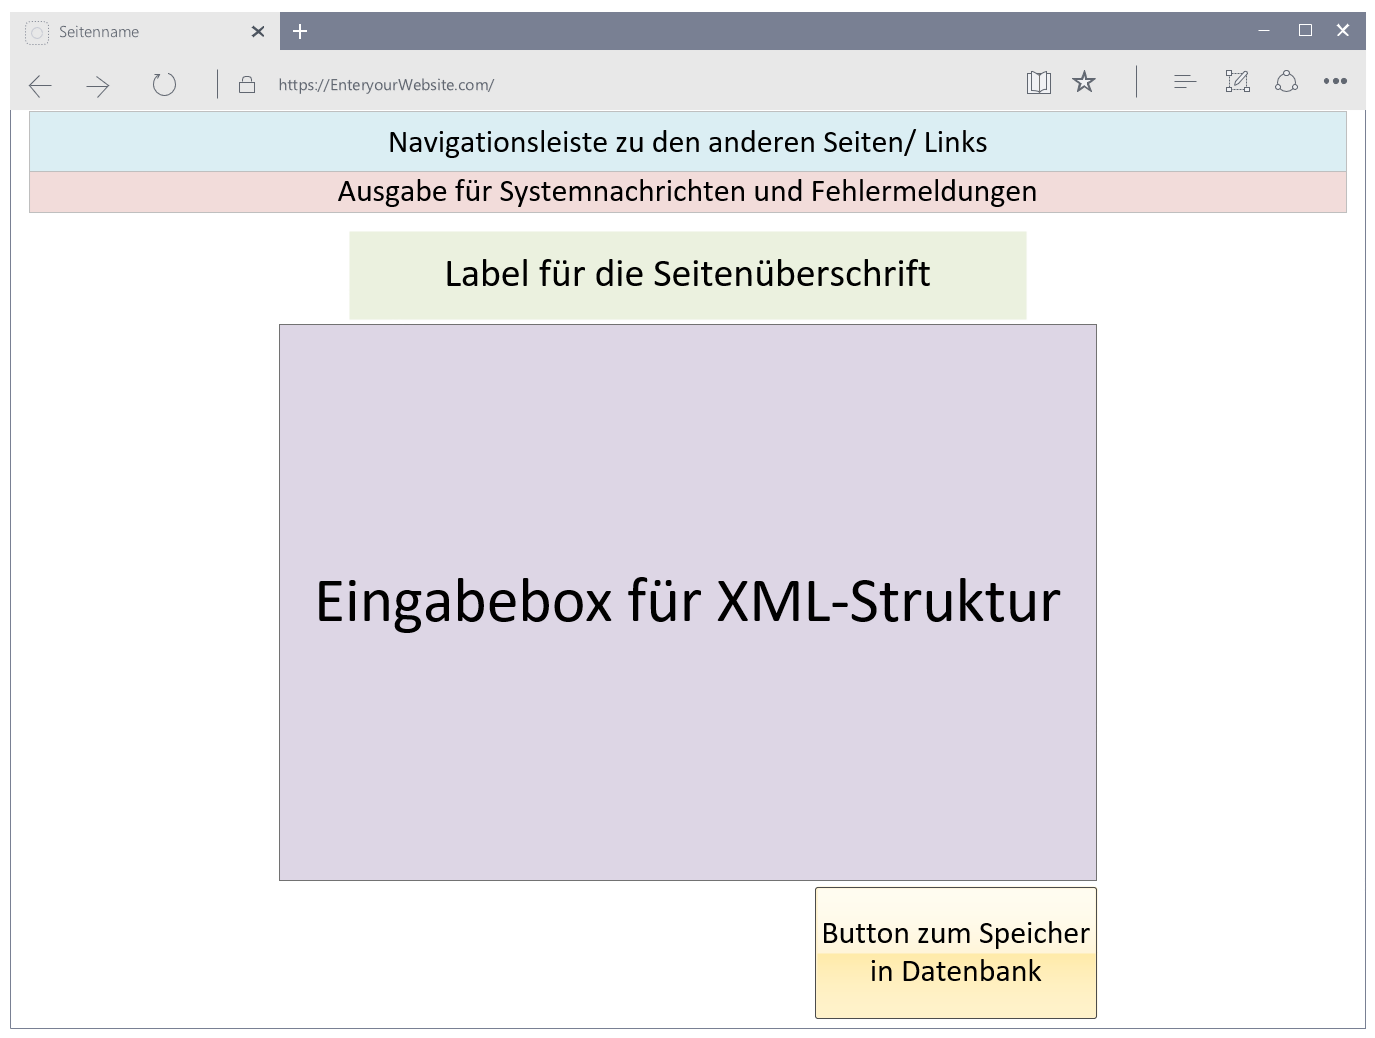
\includegraphics[width=0.95\textwidth]{Grafiken/Overlay_Einleseseite}
    \caption{Benutzeroberflächenentwurf der Seite zum Einlesen der XML-Struktur}
    \label{fig: Benutzeroberflächenentwurf der Seite zum Einlesen der XML-Struktur}
    {Quelle: Eigene Darstellung mit Microsoft Visio}
\end{figure}

Die Seite für das Darstellen und Auswählen zu visualisierenden Daten soll im oberen Abschnitt der Seite
ein Bereich für Filtereinstellungen besitzen, mit möglichen Filteroption wie Datum oder Seriennummer.
Neben dem Filtereinstellung soll zwei Button für das Bestätigen und Zurücksetzen der Filtereinstellungen
sein. Bei einem Fehler bei der Filtereingaben soll in Bereich für Systemnachrichten eine Fehlermeldung
mit möglicher Lösung erscheinen.
Im unteren Bereich der Seite soll sich eine Tabelle, welche die eingelesenen Berichte in der Datenbank
anzeigt. Diese soll durch die Filtereinstellungen angepasst werden. Hierbei muss auf eine Anzeige
Möglichkeit für länge Tabellenstrukturen berücksichtigt werden, um die Benutzung effizient zu halten. Das
Grundkonzept ist in Abbildung \ref{fig: Benutzeroberflächenentwurf der Seite zum Ausgeben der Berichtstabelle} dargestellt.

\begin{figure}[H]
    \centering
    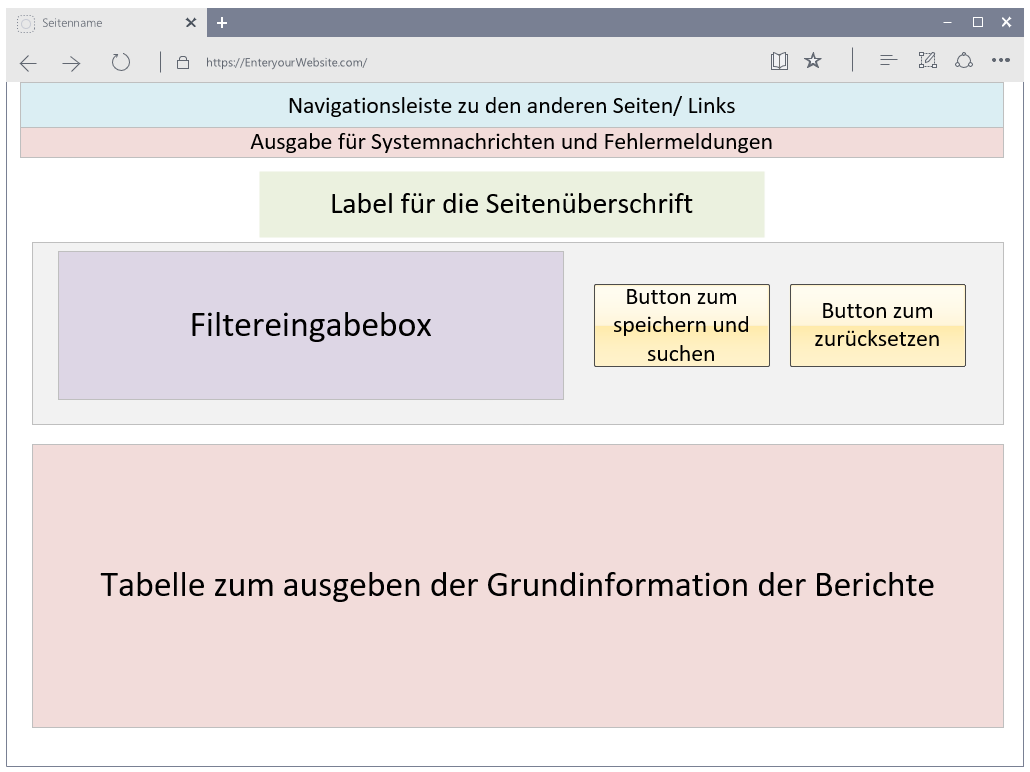
\includegraphics[width=0.95\textwidth]{Grafiken/Overlay_Tabellenseite}
    \caption{Benutzeroberflächenentwurf der Seite zum Ausgeben der Berichtstabelle}
    \label{fig: Benutzeroberflächenentwurf der Seite zum Ausgeben der Berichtstabelle}
    {Quelle: Eigene Darstellung mit Microsoft Visio}
\end{figure}

Für das Ausgeben der ausgewallten Berichtsdaten soll im oberen Abschnitt der Seite eine Instanz
eingefügt werden, die die Information zu dem Ausgewählten Berichtsdaten angezeigt werden.
Im unteren Bereich soll ein Label für die Seriennummer der Ausgewählten Berichtsdaten eingefügt
werden. Darunter werden Enthalten den Modulen mit Labeln benannt und unter den Modulname werden
die Graphen und Werte für die visuelle Darstellung der Testdaten eingefügt. Die Anzahl der Darstellungen
hängt von den in den Bericht Daten enthaltenden Modulen ab. Die Anzahl und der Aufbau des Unteren
Bereiches ist variabel. Der grundlegende Aufbau dieser Seite ist in der Abbildung \ref{fig: Benutzeroberflächenentwurf der Seite zum Ausgeben der Graphen} dargestellt.

\begin{figure}[H]
    \centering
    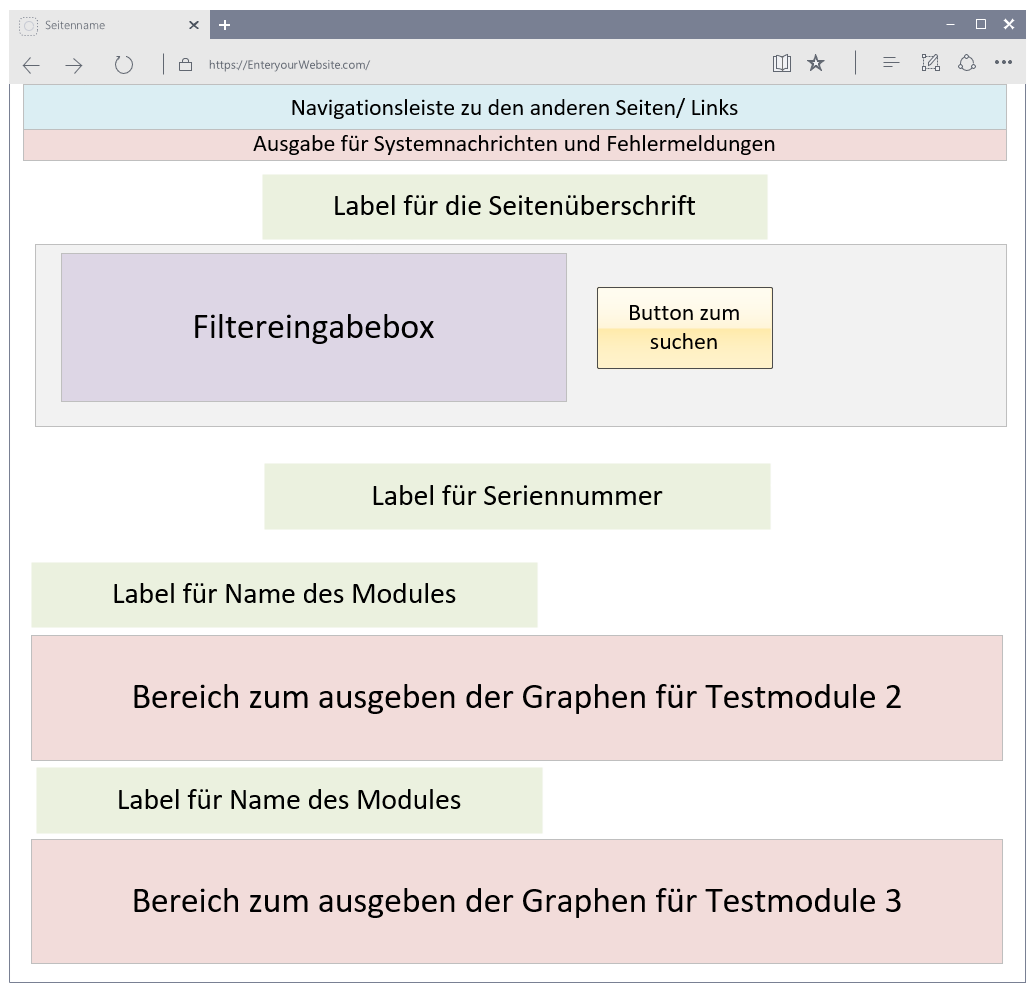
\includegraphics[width=0.95\textwidth]{Grafiken/Overlay_Ausgabeseite}
    \caption{Benutzeroberflächenentwurf der Seite zum Ausgeben der Graphen}
    \label{fig: Benutzeroberflächenentwurf der Seite zum Ausgeben der Graphen}
    {Quelle: Eigene Darstellung mit Microsoft Visio}
\end{figure}